\documentclass[11pt]{article}
\usepackage{amsmath}

\usepackage{natbib}
\bibliographystyle{agsm}

\usepackage{mathptmx} % times new roman
\usepackage[margin=2cm]{geometry}% margin
\usepackage{titlesec}

% draw sub-figures
\usepackage{caption}
\usepackage{subcaption}
\usepackage{graphicx}
\captionsetup[subfigure]{labelformat=empty}

% change heading color
\usepackage[dvipsnames]{xcolor}
\usepackage{sectsty}
\sectionfont{\color{NavyBlue}}
\subsectionfont{\color{NavyBlue}}

% column change lane
\newcommand{\specialcell}[2][c]{%
	\begin{tabular}[#1]{@{}c@{}}#2\end{tabular}}
\newcommand{\specialcelll}[2][c]{%
	\begin{tabular}[#1]{@{}l@{}}#2\end{tabular}}

\usepackage{float} %for table fixing position

% Set formats for each heading level
\usepackage{etoolbox}% http://ctan.org/pkg/etoolbox
\makeatletter
%\patchcmd{<cmd>}{<search>}{<replace>}{<success>}{<failure>}
\patchcmd{\@makechapterhead}{\large}{\small}{}{}% for \chapter
\patchcmd{\@makechapterhead}{\Large}{\small}{}{}% for \chapter
\patchcmd{\@makeschapterhead}{\normalsize}{\small}{}{}% for \chapter*
\patchcmd{\@makessectionhead}{\Large}{\small}{}{}
\patchcmd{\@makessectionhead}{\large}{\small}{}{}
\patchcmd{\@makessectionhead}{\normalsize}{\small}{}{}
\patchcmd{\@makessubsectionhead}{\Large}{\small}{}{}
\patchcmd{\@makessubsectionhead}{\large}{\small}{}{}
\patchcmd{\@makesssubectionhead}{\normalsize}{\small}{}{}

\patchcmd{\@makechapterhead}{\bfseries}{\relax}{}{}% Non-bold \chapter name
\patchcmd{\@makechapterhead}{\bfseries}{\relax}{}{}% Non-bold \chapter title
\patchcmd{\section}{\bfseries}{\relax}{}{}% Non-bold \section
\patchcmd{\subsection}{\bfseries}{\relax}{}{}% Non-bold \subsection
\makeatother

% bond under math

\usepackage{bm}

\title{What explains the volatility of the ASX 200 index? \\ Evidence from local economic conditions and \\global market performance \footnote{This report is an empirical research assignment submitted to course ECON90011(Quantitative Analysis of Finance II) at the University of Melborune.}}
\author{Zelin Chen, Yuwen Mao, Haibin Miao\\
		(Group 8)\footnote{Student ID of each author: Zelin Chen (797036), Yuwen Mao (846785) and Haibin Miao (806292). }}

\date{\today}

\begin{document} 
	\maketitle
\begin{abstract}
This paper is mainly inspired by \emph{The Spline-Garch Model for Low-Frequency Volatility and Its Global Macroeconomic Causes} \citep{Spline} and \emph{Modelling Australian Stock Market Volatility: A Multivariate GARCH Approach} \citep{index}. Two models are proposed to investigate the impact of local economic conditions (bond yields, exchange rates and unemployment rate) and global market performances (FTSE 100, NIKKEI 225 and S\&P 500) on the volatility of ASX 200 index. The GARCH(1,1) model with the conditional volatility of exogenous variables explains the average correlation of ASX 200 index volatility with risks from different aspects across periods. In addition, the MGARCH model is leveraged to provide insights in time variant conditional covariance between those variables from a historical perspective. 
\end{abstract}
\newpage

\section{Introduction}
Two of the most important elements in asset pricing, portfolio management and risk management are volatilities and correlations. Initially the univariate autoregressive conditional heteroscedasticity (ARCH) was the central focus, however, as time pass by and the improvement of computing power, the multivariate version of ARCH/GARCH models have been developed and proved to be more important and necessary which would continue to be the trend thereafter. Multivariate GARCH model, which is one of the most important models for volatility, allows people to specify a dynamic process for the whole time varying variance-covariance matrix of the time series. The MGARCH model has been extensively applied in portfolio management, option pricing, analysis of volatility spillovers across markets, hedging, conditional CAPM and Value-at-Risk (VaR) of portfolios. In addition, based on the fact that correlations between asset returns and markets are critical in many financial applications, the multivariate volatility models have also recently been extended to describe the time-varying feature of the correlations. Based on the recent theoretical and empirical development of the model, this paper is aimed to use both GARCH and multivariate GARCH model to explain and analyse the volatility of Australia Stock Market 200 Index.

This paper is organized as follows: section 2 reviews some of the applied research papers on the volatility of the ASX 200, which is the same topic this paper focuses on, including \emph{Causality of Weather Conditions in Australians Stock Equity Returns} \citep{Weather}, \emph{Effects of Exchange Rate Volatility on Stock Market Return Volatility: Evidence from an Emerging Market} \citep{exr}, \emph{The Spline-Garch Model for Low-Frequency Volatility and Its Global Macroeconomic Causes} \citep{Spline}, \emph{Modelling Australian Stock Market Volatility: A Multivariate GARCH Approach} \citep{index}, and \emph{Oil price shocks and volatility in Australian stock returns} \citep{oil}.
Section 3 briefly describes the features of the ASX 200 data, and followed by that, section 4 applies two models to the ASX data, including firstly the GARCH(1,1) with exogenous variables and secondly the multivariate GARCH model along with those exogenous variables, which forms the basis of our analysis. Section 4 presents the estimation results and empirical findings of those two models and our conclusion will be included in the last section. 

\section{Literature review}	
\cite{Spline} observed the correlation of low-frequency volatility of market return and macroeconomic variables (GDP, CPI, exchange rate and short-term interest rates) from cross-sectional analysis. The low-frequency volatility is used to match the frequency of macroeconomic indicators. They used modified component GARCH model to separate daily volatility process into two components, one with transitory shocks, the other with more permanent shocks, and then to use annualised low-frequency volatility for a country in a certain year to conduct OLS regression on a set of macroeconomic variables. We investigate those variables, but differently at monthly frequency, in our regression analysis. Because, first, our the sample size is not large enough to conduct analysis in annual frequency compared to the paper. Second, monthly is the usual minimal frequency for macroeconomic data announcement. So our data may also reveal low-frequency components, it is possible to have a try. 

\cite{exr} revealed daily impact of exchange rate volatility on Siri Lanka’s stock exchange index as an emerging market example. The return equation is consistent with rate of change of US Dollars, British Pounds and Euros. An adjusted GARCH(1,1) model is used to regress conditional variance of index volatility. It includes, in addition to its original components, volatility of Dollars, Pounds and Euros. The empirical evidence showed that only Euros had significant impact on the index, and more important, it is believed that the result is more robust for an emerging market which does not have derivative market for investors to hedge foreign exchange risks. We gained the insights that exchange rate may be an important variable to investigate when we study the volatility of ASX 200 index. Because, trades play significant role in Australia GDP. Any changes in exchange rate, through the change of trades, may have an impact on the overall economic performance, and on ASX 200 index. Different from this research, we consider to include only one index of exchange rate, the trade weighted index (TWI), into our model, since this index reveals a general measurement of how exchange rate of AUD changes against a bunch of weight trading currencies. 

\cite{index} used MGARCH model to quantify correlations between stock market returns of Australia (AORD), Singapore (STI), the UK (FTSE100) and the US (S\&P 500). Data is analysed on weekly frequency. A VAR process is used to model conditional mean equation. Authors used VECH model to solve conditional variance and covariance matrix. Because of small dimensions, VECH is not computationally burden in this case. However, as authors mentioned, the validity of estimations is restricted to the positive semi-definiteness of the conditional variance and covariance matrix. The covariance model they selected was VECH(1,1), due to its consistent lowest information criteria. Moreover, authors found no evidence for significant correlation between conditional market volatility and expected returns. We decide to follow the approach of this paper. Because, primarily, foreign market indices are always first considered when searching for correlated factors on ASX 200 index. This paper provides academic guidance for our application of these variables. Second, although MGARCH did not play a role in analysis weekly volatilities, it is worthwhile to have a try on monthly data. Because week data may reflect more transitory shocks than monthly data, while transitory shocks may not have a strong inter-market impact compared to long-term shocks. Monthly data may be more likely to capture this effect. One limitation with the application of this paper is that we can only find working paper edition available on the internet, although it has uploaded since 2008. But, at least, it has been cited by two published paper, which somehow approved its credibility. 

\cite{Weather} investigated causality of weather condition on the ASX 200 Index. They used Sydney local meteorological data, including temperatures, humidity, pressure and vapour pressure, to model Australian stock returns, and found that the humidity has significant impact on ASX 200 index. Weather variables and its lags is introduced in AR model when determine granger causalities. Each weather variable is investigated separately, and only humidity is found to be significant. The conditional variance model is simply GARCH(1,1). We decide to not introduce this finding to our report, since, first, the impact of weather on financial returns is still on huge debate, and many literatures have not found such correlation. Second, although humidity grander causes change of ASX 200 returns, with the variable itself, it is not strong enough to capture all the variations in our data. Third, we don’t have access to Sydney humidity data from Bureau of Meteorology. 

\cite{oil} studied the effect of oil shock on the return and volatility of ASX 200 index and the sectors in Australian stock market. GARCH-M model is introduced to regress market returns. The conditional mean equation of returns is consisted of its own lag, old price return, oil price return volatility, and the conditional volatility measure of returns. The conditional covariance matrix is constructed by squared past residuals, lagged conditional variance and oil return volatility. They also have a GARCH(1,1) for modelling oil price volatility. This paper inspired us on how we can add exogenous volatility variables into GARCH model. 


\section{Data description}
\begin{figure}[H]
	\centering
	\begin{subfigure}[t]{0.45\textwidth}
		\centering	
		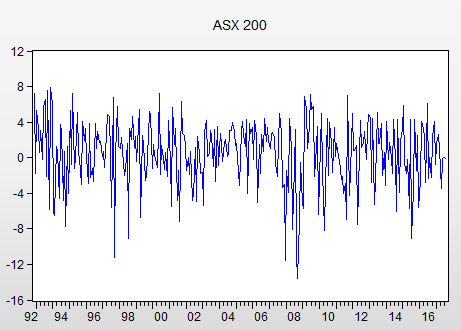
\includegraphics[width=\textwidth]{asx200.png}
	\end{subfigure}
	\hfill
	\begin{subfigure}[t]{0.45\textwidth}
		\centering
		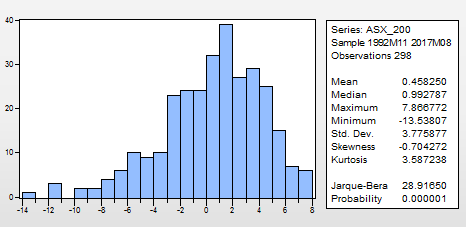
\includegraphics[width=\textwidth]{asx_sample_stats.png}
	\end{subfigure}
	\caption{Figure and Sample Statistics of ASX 200 Index}
	\label{data}
\end{figure}
Figure \ref{data} shows monthly equity return rate for ASX 200 index over the period November 1992 to August 2017. ASX 200 index is a market-capitalization weighted and float-adjusted stock market index of Australian stocks. The rate of return is calculated from monthly data with the following equation.
\[ r_{a,t} = 100 * (logP_t - logP_{t-1}) \]
Where $P_t$ is the monthly closing value for ASX 200 index.

The distribution of monthly return rate and descriptive statistics are also shown in Figure \ref{data}. It displays that the mean of monthly return rate is 0.458\% and the monthly rate of return hovers around the mean. The maximum monthly return rate is 7.867\% and the minimum return rate is -13.538\%. The figure of the monthly return rate shows that the variance of return rate varies over this period. The variance became larger during crisis periods such as the Asian Finance Crisis in 1997 and the Global Finance Crisis in 2008 due to extreme negative return rate. The probability that extreme monthly rate of return happens is also larger during these periods. The skewness of the return rate distribution is -0.704, showing that there is a larger concentration of returns below the sample mean than that above the sample mean, which is consistent with the discovery that there are more extreme negative rates than extreme positive rates. The kurtosis of 3.587 is greater than 3, indicating that the distribution exhibits more extreme return relative to a normal distribution. The JB statistic also proves that the return rate distribution does not follow a normal distribution.

\begin{table}[H]
	\centering
	\caption{Sample Statistics of Exogenous Variables}
	\begin{tabular}{l l c c c c c c c c  c}
		\hline\hline 
		variable &&	mean && std.dev && skewness && kurtosis && unit-root test \\
		\hline
		ASX 200		&& 0.458  && 3.776  && -0.704 && 3.587 && passed \\
		Bond 		&&	-0.392 && 4.714 && 0.226 && 4.051 && passed \\	
		TWI 		&&	0.083 && 2.724 && 0.226  && 5.436 && passed \\
		Unemployment &&	-0.227 && 2.667 && 0.329 && 3.115 && passed \\
		FTSE 100 	&&	0.345 && 3.933 && -0.726 && 3.866 && passed \\
		NIKKEI 225 	&&	0.028 && 5.845 && -0.561 && 4.112 && passed \\
		S\&P 500 	&&	0.584 && 4.175 && -0.869 && 4.912 && passed \\
		\hline
		\multicolumn{7}{l}{{\footnotesize \textit{Notes:} Unit root test is passed if its p-value for ADF-test $<0.05$.}}	
	\end{tabular}
	\label{tab:exo}
\end{table}
We focus our study on the factors that explains the time-varying volatility of the ASX 200 index. First of all, we use the GARCH model with exogenous variables to figure out the effect of error term and conditional variance of ASX 200 index, exogenous variables in the previous time periods on the current conditional variance. Then we figure out the covariance of AXS 200 index with other exogenous variables using the multivariable GARCH model. We firstly take the stock market indices of the US, the UK and Japan into consideration. Secondly, we try to find the connectedness between ASX 200 index and macroeconomic variables (exchange rate, bond yields and unemployment rate).\footnote{Since we did not find monthly data for GDP, we decide to include unemployment rate as an negative correlated indicator of GDP for economic performance.} The plot and sample statistics of other exogenous variables are displayed in Figure \ref{fig:exo} and Table \ref{tab:exo}, each variable is calculated in the same method as ASX 200 index.\footnote{Each is calculate for its difference in log returns, and then multiplied by 100. } There is one limitation with the unemployment variable that its data is only available up to April 2017, and the whole sample size has to be truncated to match the length of unemployment data. Fortunately, compared to the sampel size of 298, losing 5 observations will not have significant impact on our estimations.
%Finally, we study the effects of other potential variables such as trading volume and commodity price.
\begin{figure}
	\centering
	\begin{subfigure}[t]{0.31\textwidth}
		\centering
		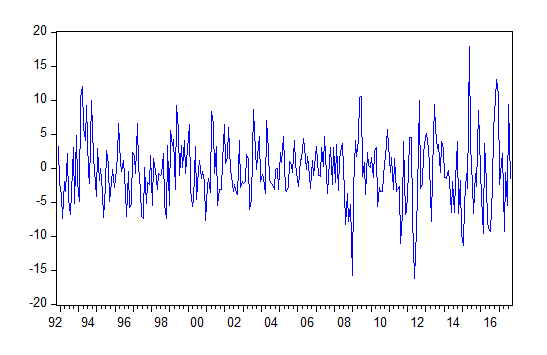
\includegraphics[width=\linewidth]{s_bond.png} 
		\caption{Bond Yields} \label{fig:sbond}
	\end{subfigure}
	\hfill
	\begin{subfigure}[t]{0.31\textwidth}
		\centering
		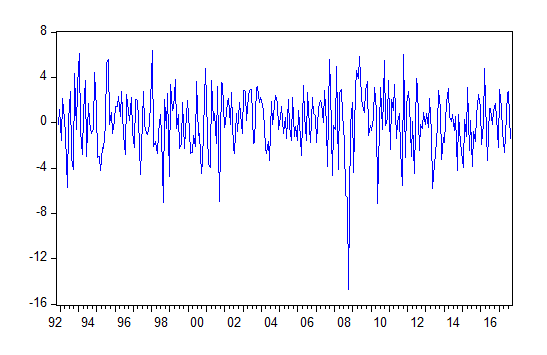
\includegraphics[width=\linewidth]{s_exr.png} 
		\caption{TWI} \label{fig:stwi}
	\end{subfigure}
	\hfill
	\begin{subfigure}[t]{0.31\textwidth}
	\centering
	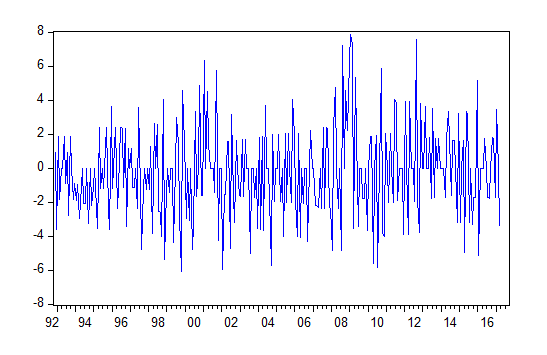
\includegraphics[width=\linewidth]{s_une.png} 
	\caption{Unemployment} \label{fig:sune}
	\end{subfigure}	

	\begin{subfigure}[t]{0.31\textwidth}
	\centering
	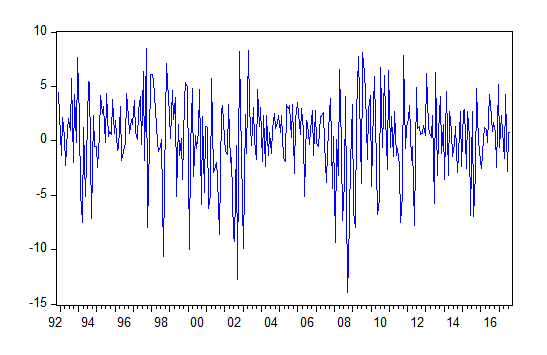
\includegraphics[width=\linewidth]{s_ftse.png} 
	\caption{FTSE 100} \label{fig:sftse}
	\end{subfigure}
	\hfill
	\begin{subfigure}[t]{0.31\textwidth}
	\centering
	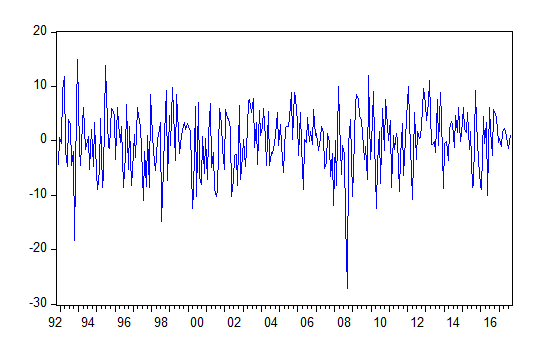
\includegraphics[width=\linewidth]{s_nik.png} 
	\caption{NIKKEI 225} \label{fig:snik}
	\end{subfigure}
	\hfill
	\begin{subfigure}[t]{0.31\textwidth}
	\centering
	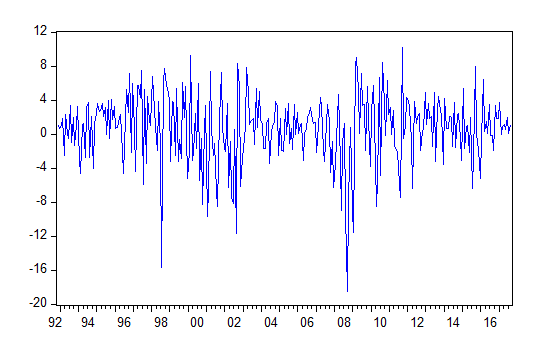
\includegraphics[width=\linewidth]{s_sp.png} 
	\caption{S\&P 500} \label{fig:ssp}
	\end{subfigure}	
	\caption{Exogenous variables in measured in logarithm difference}
\label{fig:exo}	
\end{figure}


\section{Model specification}
In order to study the conditional variance of monthly rate of return of ASX 200 index varies with GARCH model, we need to ensure that this time series data is stationary by taking the unit root test of it. The result of the unit root test is summarised shown in Table \ref{tab:exo}. The null hypothesis that this time series data has a unit root is rejected at the 1\% significance level so that the time series ASX 200 index is considered to be stationary over this period. 
Moveover, we also checked stationarity condition for exogenous variables, since they are all first differenced from their level value, it is not surprising to observe that non of them has unit root. 
On the basis of stationarity conditions, we can step further into our model specifications. 

\subsection{GARCH approach}
The first model for explaining the volatility of ASX 200 index is the GARCH(1,1) model with explanatory variables. It is inspired by \cite{Spline}, \cite{exr} and \cite{oil}. From the correlogram of returns of ASX 200 index, we see that both autocorrelation and partial autocorrelation are located in its confidence band, which indicates that it does not have any ARMA pattern. Under univariate stituation, we include only a constant and a residual term to the mean equation.\footnote{Seasonal pattern are tested, and we found that none of them is  statistically significant. }
The variance equation has a traditional GARCH(1,1) component\footnote{GARCH(1,1) is revealed by its squared residuals.}, and exogenous variables that explains volatility of economic performance and global market conditions. They are specified as following:
\begin{equation}
	r_{a,t} = c + u_{a,t}, \ \text{where} \	u_{a,t} \sim N(0,\sigma_{a,t}^2) 
\end{equation}
\begin{equation}
	\sigma_{a,t}^2 = \beta_0 + \beta_1 u_{a,t-1}^2 + \beta_2 \sigma_{a,t-1}^2 + 
	\gamma_1 Vol twi_{t} + \gamma_2 Vol bond_{t} + \gamma_3 Vol une_{t} \\
	+ \theta_1 Vol ftse_{t} + \theta_2 Volnik_{t} + \theta_3 Volsp_{t} + w_{t} 	
\end{equation}	
$r_{a,t}$ is the first difference of logarithm of ASX 200 index, which indicates monthly rate fo change of ASX 200 index. $c$ is the constant and $u_{a,t}$ is the residual. $\sigma_{a,t}^2$ is the conditional variance of ASX 200 index at time $t$, and it is consisted of squared innovation shock $u_{a,t-1}^2$ from last period and its lag-1 term $\sigma_{a,t-1}^2$. Moreover, economic variables and global market conditionas also have an impact on the volatility. $Voltwi_t$ is the conditional volatility of trade weight index of Australia exchange rate, $Volbond_t$ is the return of rate of 10-year bond, $Volume_t$ is the volatility of monthly unemployment rate, $Volftse_t$ is the conditional volatility of UK FTSE 100 index, $Volnik_t$ is the conditional volatility of Japan Nikkei 225 index, and $Volsp_t$ is the US S\& P 500 index. 
The residual in time $t$ is assumed to be randomly generated from a normal distribution with mean of zero and time-variant variance $\sigma_{t}^2$. 

\subsection{MGARCH approach}
We constructed our multivariate GARCH model  based on the findings of two papers \emph{The Spline-Garch Model for Low-Frequency Volatility and Its Global Macroeconomic Causes} \citep{Spline} and \emph{Modelling Australian Stock Market Volatility: A Multivariate GARCH Approach} \citep{index}, which respectively concluded that GDP, interest rates and inflation rates were the primary causes of market volatility and that Australian stock market was correlated with Singapore(STI), UK(FTSE100) and US (S\&P 500). However, we did some modifications when selecting data for our model for the reason that firstly monthly GDP and inflation rate data are not freely accessible from the internet. We replaced GDP and inflation with bond yield rate, exchange rate and unemployment rate considering their economic relationship and previous empirical evidence. Secondly, instead of using Singapore stock market as variables, we choose Japan (NIKKEI) as it is more representative for Asian countries and it is the second largest trading partnership with Australia.\footnote{The sources for our economic variables are from RBA official website. We did not select China index because China's share market is not fully open to oversea investors, it may not have a direct connection with global share markets.} 
%%%%% model set???????
The model follows a constant term for the mean equation, and a VECH model for the conditional covariance matrix.
\begin{align}
\bm{r_{t}} &= \bm{c} + \bm{u_{t}}, \ \text{where} \	\bm{u_{t}} \sim N(0,\bm{H_t}) \\
vech(\bm{H_t}) &= \bm{M} + \bm{A} vech(\bm{u_t u_t^{'}}) + \bm{B} vech(\bm{H_{t-1}})
\end{align}
where $\bm{r_{t}}$ is a $7\times 1$ vector indicates the returns of each variable we included in the system. $\bm{c}$ is a vector of constant, and $\bm{u_t}$ is a vector of residuals. $\bm{M}$ is a vector of constant, $\bm{A}$ and $\bm{B}$ are vectors capture lagged disturbances and lagged conditional covariance respectively.

\section{Results}
\subsection{GARCH model}
%% what paper is used?
Each exogenous variables are regressed on GARCH(1,1) model in order to predict their conditional variance across time. Then we include those predicted volatilities into our GARCH(1,1) model with exogenous variables for ASX 200 index.
\footnote{The mean equation for the GARCH of each exogenous variable includes only a constant term, because we want to keep the mean equation simple, and do not over-reduce its volatility. Each variable's GARCH model is checked for its correlogram of residuals and squared residuals, and most exogenous variables present no autocorrelations in both correlograms, except the model for bond and unemployment rate. They both have a potential MA component in their mean equation.} 
The regression result is shown in Table \ref{garch}.
\begin{table}[H]
	\centering
	\caption{GARCH(1,1) with Exogenous Variables}
	\begin{tabular}{l l l c c c c}
		\hline\hline 
			&&	variable && coefficient && t-statistic \\
		 mean equation 		&& Constant 	&& 0.766* && 4.705    \\
		 \cline{1-2}   		&&&&&& \\		 		
		variance equation   && Constant && 3.638* && 8.761 \\  
		\cline{1-2}  		&& $\text{Resid}^2$ && 0.035 	 && 1.542 \\
		 			  		&& GARCH(-1) && 1.012* && 41.10  \\
		 			  		&& TWI && 0.038* 	 && 0.400  \\  
		 			  		&& Bond && -0.027*   && 3.284 \\
		 			  		&& Unemploy&& 0.001 && 0.126 \\
		 			  		&& FTSE 100&& -0.064* 	&& 2.294 \\  
		 			  		&& Nikkei 225&& -0.107* && 11.16 \\
		 			  		&& S\&P 500&& 0.029* && 1.981 \\
		\hline
		\multicolumn{7}{l}{{ \specialcelll[l] {\footnotesize \textit{Notes:} Coefficients are marked with * if their p-value $<0.05$. t-statistics are\\ \footnotesize  reported in real values.}}	}
	\end{tabular}
	\label{garch}
\end{table}
The GARCH component lagged variance has a statistically significant impact on the ASX 200 index's current period volatility, on the other hand, the ARCH component is not significant. In addition, we found that the volatility of 10-year bond yield rate has a negative relationship with the ASX 200 Index. It is known that shares and bonds are substitutes to some extent, if the bond market is too volatile, it is probably due to hot money outflow from ASX, and invest in bond market, it results in lower volatility of ASX 200 index. We also find that the volatility of unemployment and exchange rate has little influence on the volatility of ASX 200 Index. 

In additional to the impact of economic conditions, volatility of global markets also played crucial role in explaining the volatility of ASX 200 Index. It is interesting to see that the volatility of Australia market is negatively correlated with Japan and the UK market, it indicates that when the volatility of ASX surges, Japan market and UK market are desirable markets for risks hedging. ASX 200 Index volatility has a positive co-movement with the US S\&P 500 index, which indicates that the US market is more related to ASX than Japan and the UK. 

Correlogram of squared residuals are checked, and no autocorrelations are found, which helps to prove that the model is well specified. One limitation of this model is that it only presents the average impact of exogenous variables (conditional variance) on the conditional variance of ASX 200 Index, however, it does not reveal a time-variant relationship in their correlations. Our MGARCH model, on the other hand, will explore more insights from this perspective.
%% a bit more

\subsection{MGARCH model}
We selected the Akaike Information Criterion (AIC), Schwarz Information Criterion (SIC) and Hannan-Quinn Information Criterion (HIC) to compare various models, including Diagonal VECH, Constant Conditional Correlation and Diagonal BEKK, the results indicate that Diagonal VECH specification has consistently the lowers AIC(37.58262), SIC(38.73816) and HIC(38.04543) with the average log-likelihood of -2.640. All the estimated coefficients relating to the volatility of ASX 200 index are reported in Table \ref{tab:mgarch}.
\begin{table}[H]
	\centering
	\caption{MGARCH coefficients for ASX 200 Index}
	\begin{tabular}{c c l c c c c c c}
		\hline\hline
		index &&variables 		&& M 		&& A1 		&& B1 	    \\
		\hline
		(1)&&ASX 200   		&& 1.875	&&	0.144*	&&	0.713*  \\
		(2)&&Bond			&& 0.017	&&	0.150*	&&	0.703*  \\
		(3)&&TWI				&& -0.215	&&	0.148*	&&	0.657*  \\
		(4)&&Unemployment	&& -0.022	&&	0.071	&&	0.723*  \\
		(5)&&FTSE 100		&& -0.054	&&	0.127*	&&	0.578   \\
		(6)&&NIKKEI 225		&&	0.722	&&	0.147	&&	0.512*  \\
		(7)&&SP 500 			&&	0.161	&&	0.165*	&&	0.772*  \\
		\hline
		\multicolumn{9}{l}{{ \specialcelll[l] {\footnotesize \textit{Notes:} Coefficients are marked with * if their p-value $<0.05$. \\  \footnotesize A1(1) represents $A_{1,1}$ in matrix $\bm{A}$, so on and so forth. }}	}
	\end{tabular}
\label{tab:mgarch}
\end{table}
%%% coefficient specification
The observation of these features motivates us to adopt this model, which is correspondent to our initial preference of model as the diagonal VECH model is constructed on the assumption that the conditional variance is influenced by the cross-lagged residuals and lagged covariance of other series and is able to present more information comparing to the other two. \footnote{We observe that the estimations of both GARCH and MGARCH had different results under Eviews 8 and Eviews 9. We report our results in Eviews 8 favour, because the results reported by Eviews 9 failed to converge after many iterations.}


Similar to the GARCH model, residuals from the MGARCH model are diagnosed under Portmanteau Autocorrelation Test, and no autocorrelations are found for ASX 200 index, which implies that the model is well specified for ASX 200 index. 

The elements in matrix M are all statistically insignificant so that the null hypothesis that these elements are equal to 0 cannot be rejected. As a result, we can consider these elements to be equal to 0.

As per the results, the coefficient of element $A_{1,1}$ is 0.1442 and it is statistically significant at 5\% significance level, suggesting that the past shocks in the Australian stock market do have an effect on its own future variance. The elements $A_{1,2}$, $A_{1,3}$ and $A_{1,4}$ measure the degree of effects of lagged innovation from bond yield rate, exchange rate and unemployment rate on the volatility of Australian stock market. The elements $A_{1,5}$, $A_{1,6}$ and $A_{1,7}$ describe the influence of lagged innovation in the British, Japanese and American stock market. The result shows that the strongest effect is between American and Australian stock market. The effect of lagged innovation on the unemployment rate is insignificant. Other variates' lagged innovations have approximately equal effect on the volatility of Australian stock market.

The element  $B_{1,1}$ is 0.7138, showing that the current variance of Australian stock market is influenced by its own past variance. This discovery is consistent with the outcome from GARCH model. The other elements in the first column of matrix B are nonzero and statistically significant, providing further evidence for the existence of positive cross market effect. The estimated coefficients of lagged variance from bond yield rate, exchange rate and unemployment rate on the volatility of Australian stock market are 0.7026, 0.6569 and 0.7230 respectively. The estimated lagged cross variance persistence between Australian stock market and British, Japanese and American stock market are 0.5781, 0.5119 and 0.7721 respectively. The lagged variance of American stock market has the most significant effect on the volatility of Australian stock market. The lagged variance of bond yield rate, unemployment rate and American stock market have relatively significant effect on the volatility of Australian stock market.

The historical connectedness between these variates from this model is shown in Figure \ref{corr}.
\begin{figure}[h]
	\centering
	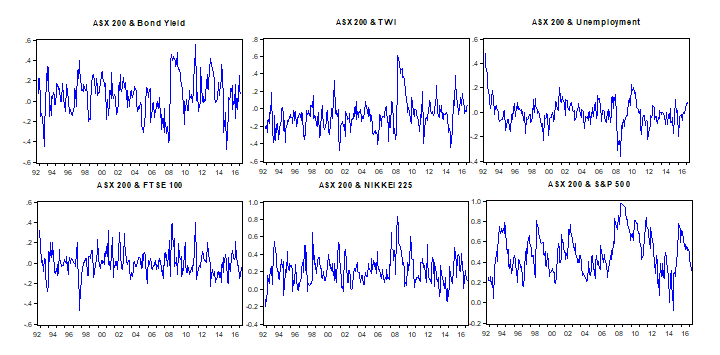
\includegraphics[width=\textwidth]{cor_asx.png}
	\caption{Conditional correlation of ASX 200 Index with other variables}
	\label{corr}	
\end{figure}
The first graph of Figure \ref{corr} shows that the correlation between Australian stock market and bond yield rate hovers around 0, however the correlation presents two spikes. The correlation becomes larger to about 0.4 during crisis period. The second graph on the right indicates that the correlation between stock market and exchange rate hovers around approximate -0.05 and it also presents a spike during GFC period to about 0.6. The third graph suggests that the correlation between stock market and unemployment rate hovers around the mean of 0. The correlation decreased to about -0.4 during GFC period and rebounded to about 0.2 after it. The fourth graph shows that the correlation between Australian and British stock market hovers 0. The correlation decreased to -0.4 during Asian Finance Crisis and increased to 0.4 during GFC period. The fifth graph indicates that the mean of correlation between Australian and Japanese stock market is approximate 0.25. The correlation remains positive over this estimate period and increases during Asian Finance Crisis and GFC periods. The bottom graph suggests that the correlation between Australian and American stock market also remains positive and hovers around the mean of about 0.5. The correlation between them increased to almost 1 during GFC period and decreased to 0 gradually after it. The correlation rebounded to 0.7 later.
We can come up with the conclusion that correlations between different segment markets in Australian financial market and stock market is roughly 0, however the correlation would increase in a large degree during crisis periods. The correlation between Australian and British stock market is approximate 0. The Australian stock market has positive correlation with both Japanese and American stock market and it has a larger correlation with American stock market. All of these correlation would increase during crisis period because all these stock markets are influenced by the finance crisis and the influence of financial crisis would disseminate across countries quickly.
 

\section{Conclusion}
To sum up, this paper generally investigates what explains the volatility spillovers of ASX 200 by applying both GARCH (1,1) with exogenous variables and multivariate GARCH model (Diagonal VECH). 
The results of GARCH(1,1) model present the convincing evidence of how the volatility of economic conditions and global markets can influence on the volatility of ASX 200 index. On average, increase of volatility of bond yields, FTSE 100 index and Nikeei 225 index have negative impact on the volatility of ASX 200. Conversely, GARCH(-1) component and the volatility of S\&P 500 are found to have positive correlation with the volatility of ASX 200 index.
The empirical findings of the multivariate GARCH model indicates that in general the volatility spillovers between ASX 200 and other indexes is more observable than with various rates, among those variables, S\&P 500 is the most obvious with average variance of 0.5 followed by NIKKEI 225. In contrast, the overall volatility and correlation contagion among ASX 200 and various rates were weak as only slightly positive correlation were detected. 

%% my conclusion

\newpage
\nocite{*}
\bibliography{ref}

	
\end{document}